\documentclass[conference]{IEEEtran}

\usepackage[T1]{fontenc}
\usepackage[utf8]{inputenc}
\usepackage{cite}
\usepackage{url}
\usepackage{booktabs}
\usepackage{amsmath}
\usepackage{graphicx}
\usepackage{hyperref}
\usepackage{stfloats}
\usepackage{array}

\newcommand{\code}[1]{\mbox{\texttt{#1}}}

\title{Interim QCar Evry Trajectory Report: Comparing Monocular SVO and Depth Anything 3 on Recorded QCar Evry Sequences}

\author{
\IEEEauthorblockN{Project Report Draft}
\IEEEauthorblockA{mono3d-benchmark Experimental Notes\\
June 12, 2026}
}

\begin{document}

\maketitle

\begin{abstract}
This interim report summarizes the first completed trajectory comparison on the recorded QCar Evry dataset inside the \texttt{mono3d-benchmark} workflow. The present study evaluates monocular SVO Pro Open~\cite{forster2017svo} and Depth Anything 3 (DA3)~\cite{lin2025depthanything3} on six logged indoor campus sequences: \code{bookstore}, \code{office0}, \code{office1}, \code{office2}, \code{warehouse1}, and \code{warehouse2}. The comparison uses three report layers: SVO versus ground truth, DA3 versus ground truth, and SVO versus the best DA3 result per sequence. Across all six sequences, DA3 wins every direct Sim(3) comparison. Mean Sim(3) RMSE decreases from 8.253~m for SVO to 3.702~m for the best DA3 run per sequence, while the median decreases from 7.005~m to 0.724~m. The main exception is \code{warehouse1}, which remains difficult for both systems and dominates the remaining DA3 error. These results are consistent with the earlier TUM finding that learned monocular priors can outperform plain monocular SVO when the input is RGB-only and non-inertial. At the same time, the report keeps the interpretation provisional: these are offline results on recorded logs, and live visual-feed testing is scheduled for next week.
\end{abstract}

\begin{IEEEkeywords}
Monocular visual odometry, learned monocular priors, SVO, Depth Anything 3, trajectory evaluation, campus robotics, QCar
\end{IEEEkeywords}

\section{Introduction}
The purpose of this note is to extend the earlier SVO-versus-DA3 analysis from benchmark datasets to the local QCar Evry recordings collected in a campus environment. The question is practical: if the next deployment target is the QCar platform, which trajectory source is currently more trustworthy in a monocular RGB-only setting?

Earlier repository results had already established two important facts. First, SVO remains effective when IMU is available, especially on EuRoC~\cite{burri2016euroc}. Second, DA3-LARGE through the DA3-Streaming pipeline can outperform plain monocular SVO on indoor RGB trajectories in TUM-style settings~\cite{sturm2012tumrgbd}. The QCar Evry dataset is therefore a useful intermediate step between public benchmark validation and the live visual-feed tests planned for next week.

The report is intentionally scoped as an interim offline study. All results below come from recorded sequences with available ground-truth poses. No claims are made yet about online robustness under a live onboard camera feed. The value of this report is that it documents the current baseline before that next stage of testing.

\section{Experimental Setup}

\subsection{Dataset}
The evaluated QCar Evry dataset contains six RGB sequences with matched ground-truth poses:
\begin{quote}
\ttfamily\small
bookstore\\
office0\\
office1\\
office2\\
warehouse1\\
warehouse2
\end{quote}

Each sequence includes an RGB stream and a \code{groundtruth.txt} file in TUM-style pose format. The current evaluation therefore focuses on trajectory estimation quality rather than solely on qualitative reconstruction appearance.

\subsection{SVO Configuration}
The SVO side uses the restored SVO Pro Open benchmark path already integrated in this repository~\cite{forster2017svo}. For QCar, the run was strictly monocular:
\begin{quote}
\ttfamily\small
use\_imu: false\\
use\_ceres\_backend: false\\
runlc: false
\end{quote}

The QCar monocular calibration written into \code{calib.yaml} uses a pinhole camera with:
\begin{quote}
\ttfamily\small
fx = fy = 695.9951\\
cx = 640.0,\; cy = 360.0\\
image size = 1280 $\times$ 720
\end{quote}

This makes the QCar SVO path comparable in spirit to the earlier TUM monocular experiments: geometry only, no inertial assistance, and no loop-closure rescue path in the final usable run.

\subsection{DA3 Configuration}
The learned baseline uses DA3-LARGE through the DA3-Streaming pipeline~\cite{lin2025depthanything3}. For each QCar sequence, the pipeline was run at:
\begin{itemize}
\item \texttt{fps} $\in \{2,3,5\}$,
\item chunk size $= 30$,
\item overlap $= 15$,
\item loop-enabled chunk alignment.
\end{itemize}

The evaluation then selected the best DA3 variant per sequence according to minimum Sim(3) RMSE against ground truth.

\subsection{Metrics}
The report follows the same trajectory metrics used in the earlier repository studies:
\begin{itemize}
\item tracking ratio,
\item trajectory ratio,
\item SE(3) RMSE,
\item Sim(3) RMSE,
\item path-ratio-to-ground-truth.
\end{itemize}

Sim(3) RMSE is emphasized because it isolates trajectory-shape fidelity after similarity alignment. As in the earlier reports, this means the Sim(3) numbers describe structural trajectory correctness rather than raw metric-scale recovery.

\section{Results}

\subsection{SVO Versus Ground Truth}
The SVO-only QCar report shows that the tracker was often active, but the resulting monocular geometry was weak. Mean tracking ratio was 0.787 and mean trajectory ratio was 0.581 across the six sequences. However, the mean Sim(3) RMSE remained 8.253~m, and the mean path-ratio-to-ground-truth was only 0.476. In other words, SVO often kept a visual lock on the sequence, but that did not translate into a geometrically reliable trajectory.

This failure mode is especially clear in \code{warehouse1}. There, SVO reached a tracking ratio of 0.664, yet its Sim(3) RMSE was still 18.879~m and its estimated-path-to-ground-truth ratio was only 0.227. This is consistent with monocular drift and scale collapse rather than total tracking failure.

\begin{figure}[t]
\centering

\includegraphics[width=\columnwidth]{../evaluation/qcar_svo_vs_gt_20260612_114149_mono3d_qcar_evry_mono/sim3_rmse.png}
\caption{QCar SVO-versus-ground-truth Sim(3) RMSE across the six recorded sequences.}
\label{fig:qcar-svo-gt-sim3}
\end{figure}

\subsection{DA3 Versus Ground Truth}
The DA3 side performed better on every QCar sequence when the best run per scene was selected from the tested \texttt{fps} settings. The strongest per-sequence DA3 choices were:
\begin{itemize}
\item \code{bookstore}: 5~fps,
\item \code{office0}: 2~fps,
\item \code{office1}: 2~fps,
\item \code{office2}: 3~fps,
\item \code{warehouse1}: 2~fps,
\item \code{warehouse2}: 3~fps.
\end{itemize}

Five of the six sequences reached sub-meter Sim(3) RMSE with the selected best DA3 variant. The clear outlier was again \code{warehouse1}, where the best DA3 run still produced 18.203~m Sim(3) RMSE. This indicates that the sequence is genuinely hard rather than merely unfavorable to SVO alone.

\begin{figure}[t]
\centering

\includegraphics[width=\columnwidth]{../evaluation/qcar_da3_vs_gt_20260612_114149_mono3d_qcar_evry_mono/sim3_rmse_best.png}
\caption{QCar DA3-versus-ground-truth Sim(3) RMSE for the best DA3 run per sequence.}
\label{fig:qcar-da3-gt-sim3}
\end{figure}

\subsection{Direct SVO Versus DA3 Comparison}
The main direct result is simple: DA3 wins all six QCar sequences in Sim(3)-aligned trajectory error. Table~\ref{tab:qcar-sequence-results} summarizes the sequence-level comparison.

\begin{table*}[!t]
\caption{QCar sequence-level Sim(3) RMSE comparison between monocular SVO and the best DA3 run per sequence}
\label{tab:qcar-sequence-results}
\centering
\small
\begin{tabular}{lcccc}
\toprule
\textbf{Sequence} & \textbf{SVO Sim(3) RMSE (m)} & \textbf{Best DA3 Sim(3) RMSE (m)} & \textbf{Best DA3 FPS} & \textbf{Winner} \\
\midrule
\texttt{bookstore}  & 9.3758  & \textbf{1.6751}  & 5 & DA3 \\
\texttt{office0}    & 6.7783  & \textbf{0.6633}  & 2 & DA3 \\
\texttt{office1}    & 7.2322  & \textbf{0.6581}  & 2 & DA3 \\
\texttt{office2}    & 3.0573  & \textbf{0.2298}  & 3 & DA3 \\
\texttt{warehouse1} & 18.8786 & \textbf{18.2035} & 2 & DA3 \\
\texttt{warehouse2} & 4.1967  & \textbf{0.7844}  & 3 & DA3 \\
\bottomrule
\end{tabular}
\end{table*}

At aggregate level:
\begin{itemize}
\item mean SVO Sim(3) RMSE: 8.253~m,
\item mean DA3 Sim(3) RMSE: 3.702~m,
\item median SVO Sim(3) RMSE: 7.005~m,
\item median DA3 Sim(3) RMSE: 0.724~m.
\end{itemize}

The median is especially revealing. DA3's median is below 1~m because five of the six scenes are solved much more cleanly than with SVO. The higher DA3 mean is largely driven by the remaining \code{warehouse1} failure case.

\begin{figure*}[!t]
\centering

\includegraphics[width=0.97\textwidth]{../evaluation/qcar_svo_vs_da3_20260612_114149_mono3d_qcar_evry_mono/sim3_rmse.png}
\caption{Direct QCar Sim(3) RMSE comparison between monocular SVO and the best DA3 run per sequence. DA3 wins every tested scene, but \texttt{warehouse1} remains difficult for both methods and dominates the residual DA3 error.}
\label{fig:qcar-svo-da3-sim3}
\end{figure*}

\section{Interpretation}

\subsection{Why SVO Underperformed Relative to EuRoC}
The QCar result should not be read as contradicting the earlier EuRoC outcome. On EuRoC, the strong SVO result was the visual-inertial one, not the plain monocular one. By contrast, the QCar study here used:
\begin{itemize}
\item no IMU,
\item no Ceres visual-inertial backend,
\item no loop closure in the final usable SVO run.
\end{itemize}

That places QCar much closer to the earlier TUM monocular setting than to the EuRoC mono+IMU setting. In a non-inertial monocular regime, SVO must recover structure from parallax and feature geometry alone. Repeated indoor appearance, long corridor motion, and weak baseline segments make this substantially harder.

\subsection{What the Current QCar Result Suggests}
The present QCar outputs reinforce the earlier TUM interpretation:
\begin{enumerate}
\item learned monocular priors can be materially better than plain monocular geometric VO when the input is RGB-only,
\item the improvement is not necessarily universal, because hard domain-specific scenes like \code{warehouse1} can still defeat both systems,
\item SVO remains useful as a geometric cross-check even when it is not the best standalone monocular estimator.
\end{enumerate}

In particular, the QCar study supports a practical design stance: if the immediate goal is offline RGB-only trajectory recovery on these campus sequences, DA3 is the stronger current option. If the goal is interpretability or failure diagnosis, SVO still adds value.

\section{Qualitative Scene Montage}
Figure~\ref{fig:qcar-topdown-montage} collects the six top-down 3D reconstruction screenshots exported from the DA3 QCar runs during manual inspection. The figure is not a replacement for the quantitative metrics. Instead, it provides a compact qualitative check on scene coherence across the current offline study: bookstore, office-scale scenes, and warehouse-scale traversals. The montage also helps connect the trajectory findings to the recovered map structure: most scenes show a coherent top-down reconstruction under DA3, while \code{warehouse1} remains visibly difficult and agrees with its high residual trajectory error.

\begin{figure*}[!t]
\centering
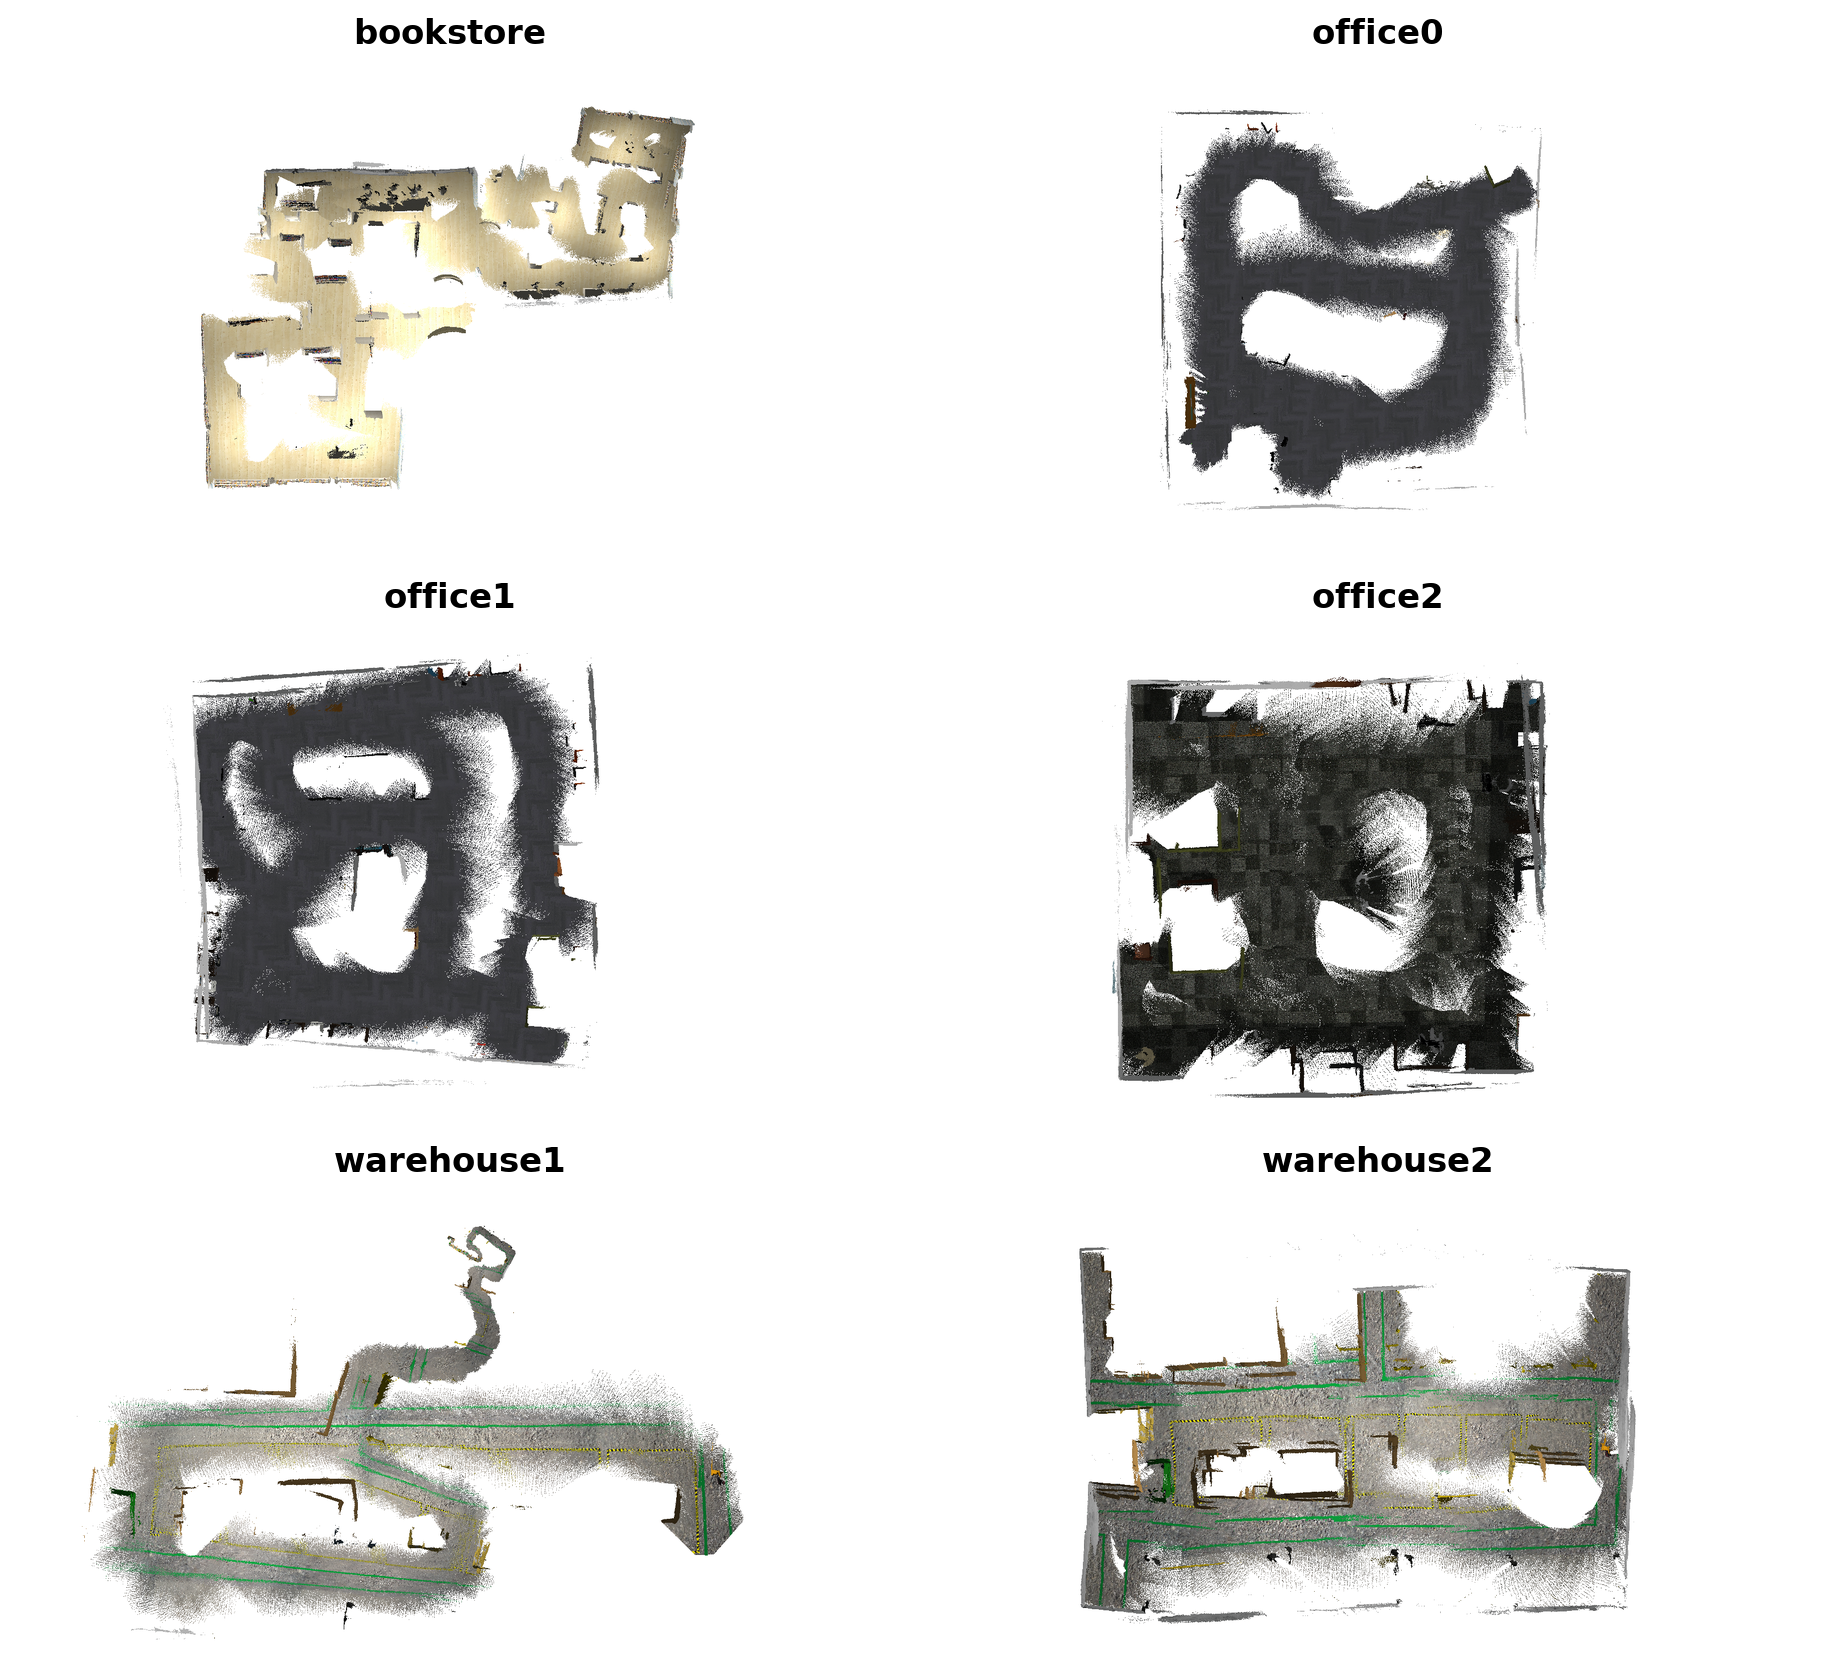
\includegraphics[width=0.92\textwidth]{figures/qcar_topdown_reconstruction_montage.png}
\caption{Two-column montage of top-down DA3 3D reconstruction screenshots across the six recorded QCar scenes: \texttt{bookstore}, \texttt{office0}, \texttt{office1}, \texttt{office2}, \texttt{warehouse1}, and \texttt{warehouse2}. These exported reconstruction views complement the CSV-based trajectory evaluation with a qualitative coherence check.}
\label{fig:qcar-topdown-montage}
\end{figure*}

\section{Status and Next Step}
This report is intentionally an interim checkpoint rather than a final deployment claim. The current outputs come from recorded QCar Evry sequences with available ground truth. They therefore answer the offline question:
\begin{quote}
Given the presently restored repository paths, which trajectory source is stronger on the logged campus data?
\end{quote}

The next stage is the live visual-feed test planned for next week. That stage matters because runtime behavior, online initialization stability, scene-entry conditions, and exposure variation can all change the ranking observed in offline replay. Until then, the present report should be read as the current best repository-backed evidence rather than as a final hardware deployment conclusion.

\section{Conclusion}
The recorded QCar Evry study supports four practical conclusions.
\begin{enumerate}
\item \textbf{DA3 is currently the stronger monocular RGB-only trajectory source on the tested QCar logs.} It wins all six direct sequence comparisons against SVO in Sim(3) RMSE.
\item \textbf{SVO remained visually active on many sequences, but tracking stability did not imply geometric reliability.} The path-ratio and Sim(3) results show substantial monocular drift and scale weakness.
\item \textbf{The earlier EuRoC result is still consistent with this outcome.} EuRoC validated SVO most strongly in the mono+IMU regime, whereas QCar here was evaluated in a strictly non-inertial monocular mode.
\item \textbf{The result should remain provisional until live-feed testing is completed.} The current evidence is strong enough to guide the next week of work, but not yet strong enough to close the full deployment question.
\end{enumerate}

Accordingly, the recommended interpretation for now is to treat DA3 as the primary offline RGB-only trajectory baseline for QCar Evry, while retaining SVO as an interpretable geometric reference and as a candidate for renewed testing once live sensing and, if possible, inertial integration are brought back into the loop.

\section*{Reproducibility Note}
The three main result folders for this report are located under \code{reports/evaluation/}:
\begin{itemize}
\item \texttt{qcar\_svo\_vs\_gt\_20260612\_114149\_mono3d\_qcar\_evry\_mono}
\item \texttt{qcar\_da3\_vs\_gt\_20260612\_114149\_mono3d\_qcar\_evry\_mono}
\item \texttt{qcar\_svo\_vs\_da3\_20260612\_114149\_mono3d\_qcar\_evry\_mono}
\end{itemize}
They contain the CSV summaries and plots referenced in this note.

\bibliographystyle{IEEEtran}
\bibliography{ieee_svo_da3_refs_2026-06-10}

\end{document}
